
%(BEGIN_QUESTION)
% Copyright 2010, Tony R. Kuphaldt, released under the Creative Commons Attribution License (v 1.0)
% This means you may do almost anything with this work of mine, so long as you give me proper credit

Determine the statuses of the red and green lamps given the following switch stimuli for this relay circuit:

$$\includegraphics[width=15.5cm]{i04770x01.eps}$$

\begin{itemize}
\item{} Applied pressure = 50 PSI
\item{} Liquid level = 1.1 feet
\item{} Process temperature = 143 $^{o}$F
\end{itemize}

\vskip 10pt

Red light = {\it energized} or {\it de-energized}?

\vskip 10pt

Green light = {\it energized} or {\it de-energized}?

\underbar{file i04770}
%(END_QUESTION)





%(BEGIN_ANSWER)

Red light = {\bf energized}

Green light = {\bf energized}

%(END_ANSWER)





%(BEGIN_NOTES)

{\bf This question is intended for exams only and not worksheets!}.

%(END_NOTES)

